\documentclass[newpage]{homework}

\input{odesII6331}
\newcommand{\hwnum}{4}

\usepackage{float}
\usepackage{booktabs}

\usepackage{tikz}
\usetikzlibrary{decorations.pathreplacing,calc}

\begin{document}
	\maketitle
	
	\question*{3.55}
	
	
	Let $y(n)$ be the number of ways to paint a strip of length $n$. Consider a strip of length $n+2$. 
	
	If the first square is blue, then the next $n+1$ squares may be painted in any way as long as no two consecutive squares are red. Thus, there are $y(n+1)$ ways to paint $n+2$ squares with the first one blue. 
	
	If the first square is red, then the next square must be blue, and the subsequent $n$ squares may be painted in any way as long as no two consecutive squares are red. Thus, there are $y(n)$ ways to paint $n+2$ squares with the first one red.
	
	The first square is either red or blue, so $y(n+2) = y(n+1) + y(n)$. The characteristic equation of this homogeneous difference equation is $0=\lambda^2 - \lambda - 1$, which has roots $\lambda_1 = \frac{1 + \sqrt{5}}{2}$ and $\lambda_2 = \frac{1-\sqrt{5}}{2}$, so
	\begin{equation*}
	y(n) = c_1\lambda_1^n + c_2\lambda_2^n = c_1\left(\frac{1+\sqrt{5}}{2}\right)^n+c_2\left(\frac{1-\sqrt{5}}{2}\right)^n
	\end{equation*}
	Since there are two ways to paint a strip of length 1, we have $y(1) = 2$. There are 3 ways to paint a strip of length 2 (red-blue, blue-red, blue-blue), so $y(2) = 3$. This implies that
	\begin{equation*}
		\begin{aligned}
			2 &= c_1\lambda_1 + c_2\lambda_2 \\
			3 &= c_1\lambda_1^2 + c_2\lambda_2^2
		\end{aligned}
	\end{equation*}
	so
	\begin{equation*}
		\begin{aligned}
			c_1 &= \frac{1}{\lambda_1\lambda_2^2 - \lambda_2\lambda_1^2}(2\lambda_2^2 - 3\lambda_2) \\
			c_2 &= \frac{1}{\lambda_1\lambda_2^2-\lambda_2\lambda_1^2}(3\lambda_1 - 2\lambda_1^2)
		\end{aligned}
	\end{equation*}
	We have $\lambda_1^2 = \frac{1+2\sqrt{5}+5}{4} = \frac{3+\sqrt{5}}{2}$ and $\lambda_2^2 = \frac{1-2\sqrt{5}+5}{4} = \frac{3-\sqrt{5}}{2}$, and therefore
	\begin{equation*}
		\begin{aligned}
			\lambda_1\lambda_2^2 - \lambda_2\lambda_1^2 &= \frac{\big(1+\sqrt{5}\big)\big(3-\sqrt{5}\big) - 		\big(1-\sqrt{5}\big)\big(3+\sqrt{5}\big)}{4} \\
			&=\frac{3+2\sqrt{5}-5-(3-2\sqrt{5}-5)}{4}=\sqrt{5}
		\end{aligned}
	\end{equation*}
	so
	\begin{equation*}
		\begin{aligned}
			c_1 &= \frac{6-2\sqrt{5}-3+3\sqrt{5}}{2\sqrt{5}} = \frac{5+3\sqrt{5}}{10}\\
			c_2 &= \frac{3+3\sqrt{5}-6 -2\sqrt{5}}{2\sqrt{5}} = \frac{5-3\sqrt{5}}{10}
		\end{aligned}
	\end{equation*}
	and
	\begin{equation*}
		y(n) = \left(\frac{5+3\sqrt{5}}{10}\right)\left(\frac{1+\sqrt{5}}{2}\right)^n + \left(\frac{5-3\sqrt{5}}{10}\right)\left(\frac{1-\sqrt{5}}{2}\right)^n
	\end{equation*}
	
	\question*{3.56}
	
	
	Let $y(n)$ be the number of ways to tile a hallway of length $n$. Consider a hallway of length $n+2$. If the first tile is a blue tile, then there are $y(n+1)$ ways to tile the remaining $n+1$ tiles. If the first tile is a red tile, then there are $y(n)$ ways to tile the remaining $n$ tiles. Therefore, $y(n+2) = y(n+1) + y(n)$. This is the same equation as in 3.55, so we get
	\begin{equation*}
		y(n) = c_1\lambda_1^n + c_2\lambda_2^n
	\end{equation*}
	for the same $\lambda_1$ and $\lambda_2$ from before but different $c_1$ and $c_2$. In particular, since there is one way to tile a hallway of length 1 (with the blue tile) and two ways to tile a hallway of length 2 (with two blue tiles or one red tile), we have $y(1) = 1$, and $y(2) = 2$. This gives
	\begin{equation*}
		\begin{aligned}
			1 &= c_1\lambda_1 + c_2\lambda_2 \\
			2 &= c_2\lambda_1^2 + c_2\lambda_2^2
		\end{aligned}
	\end{equation*}
	so
	\begin{equation*}
		\begin{aligned}
			c_1 &= \frac{1}{\lambda_1\lambda_2^2 - \lambda_2\lambda_1^2}(\lambda_2^2 - 2\lambda_2)\\
			c_2 &= \frac{1}{\lambda_1\lambda_2^2 - \lambda_2\lambda_1^2}(2\lambda_1 - \lambda_1^2)
		\end{aligned}
	\end{equation*}
	Using the calculations from 3.55, we get
	\begin{equation*}
		\begin{aligned}
			c_1 &= \frac{3-\sqrt{5} - 2 + 2\sqrt{5}}{2\sqrt{5}}=\frac{5 + \sqrt{5}}{10}\\
			c_2 &=\frac{2+2\sqrt{5} - 3 -\sqrt{5}}{2\sqrt{5}} =\frac{5-\sqrt{5}}{10}
		\end{aligned}
	\end{equation*}
	and
	\begin{equation*}
		y(n) = \left(\frac{5 + \sqrt{5}}{10}\right)\left(\frac{1+\sqrt{5}}{2}\right)^n + 	\left(\frac{5-\sqrt{5}}{10}\right)\left(\frac{1-\sqrt{5}}{2}\right)^n
	\end{equation*}
	
	\question*{3.74}
	
	\begin{alphaparts}
		\questionpart
		Let a $y$-hallway of length $n$ be a $2\times n$ hallway on top of a $2\times(n-1)$ hallway with the extra two squares on top being on the left end, as below (Figure 1). Let $y(n)$ be the number of tilings of a $y$-hallway of length $n$.
		\begin{figure}[H]
			\centering
			
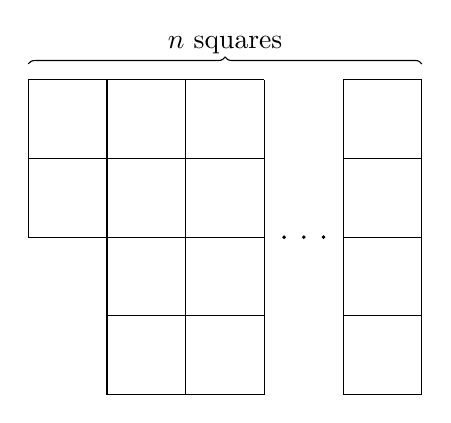
\begin{tikzpicture}
	
	\draw (1,0) -- (3,0);
	\draw (1,1) -- (3,1);
	\draw (0,2) -- (3,2);
	\draw (0,3) -- (3,3);
	\draw (0,4) -- (3,4);
	
	\draw (0,2) -- (0,4);
	\draw (1,0) -- (1,4);
	\draw (2,0) -- (2,4);
	\draw (3,0) -- (3,4);
	
	\fill (3.25, 2) ellipse (.025 and .025);
	\fill (3.5,2) ellipse (.025 and .025);
	\fill (3.75, 2) ellipse (.025 and .025);
	
	\draw (4,0) -- (4,4);
	\draw (5,0) -- (5,4);
	
	\draw (4,0) -- (5,0);
	\draw (4,1) -- (5,1);
	\draw (4,2) -- (5,2);
	\draw (4,3) -- (5,3);
	\draw (4,4) -- (5,4);
	
	
	\draw [decorate, decoration={brace}] (0,4.2) -- node [midway, anchor=south] {$n$ squares} (5,4.2);
\end{tikzpicture}
			\caption{A $y$-hallway of length $n$.}
		\end{figure}
		Let a $z$-hallway of length $n$ be a $2\times n$ hallway with two $1\times (n-1)$ halways on top and bottom, with the extra two squares in the middle hanging out to the left, as below (Figure 2). Let $z(n)$ be the number of tilings of a $z$-hallway of length $n$.
		\begin{figure}[H]
			\centering
			
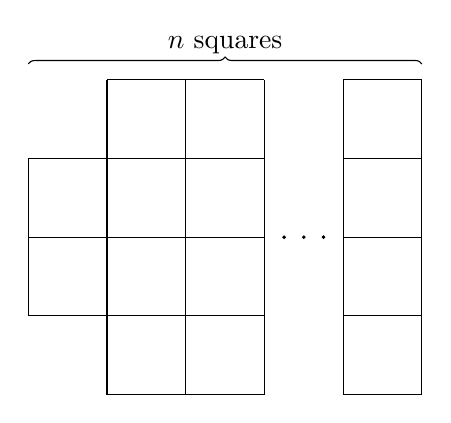
\begin{tikzpicture}
	
	\draw (1,0) -- (3,0);
	\draw (0,1) -- (3,1);
	\draw (0,2) -- (3,2);
	\draw (0,3) -- (3,3);
	\draw (1,4) -- (3,4);
	
	\draw (0,1) -- (0,3);
	\draw (1,0) -- (1,4);
	\draw (2,0) -- (2,4);
	\draw (3,0) -- (3,4);
	
	\fill (3.25, 2) ellipse (.025 and .025);
	\fill (3.5,2) ellipse (.025 and .025);
	\fill (3.75, 2) ellipse (.025 and .025);
	
	\draw (4,0) -- (4,4);
	\draw (5,0) -- (5,4);
	
	\draw (4,0) -- (5,0);
	\draw (4,1) -- (5,1);
	\draw (4,2) -- (5,2);
	\draw (4,3) -- (5,3);
	\draw (4,4) -- (5,4);
	
	
	\draw [decorate, decoration={brace}] (0,4.2) -- node [midway, anchor=south] {$n$ squares} (5,4.2);
\end{tikzpicture}
			\caption{A $z$-hallway of length $n$.}
		\end{figure}
		Now consider a $4 \times (n+2)$ hallway. The leftmost two columns of every tiling of this hallway must look like one and only one of the four possibilities below, where the shaded areas represent tiles.
		\begin{figure}[H]
			\centering
			
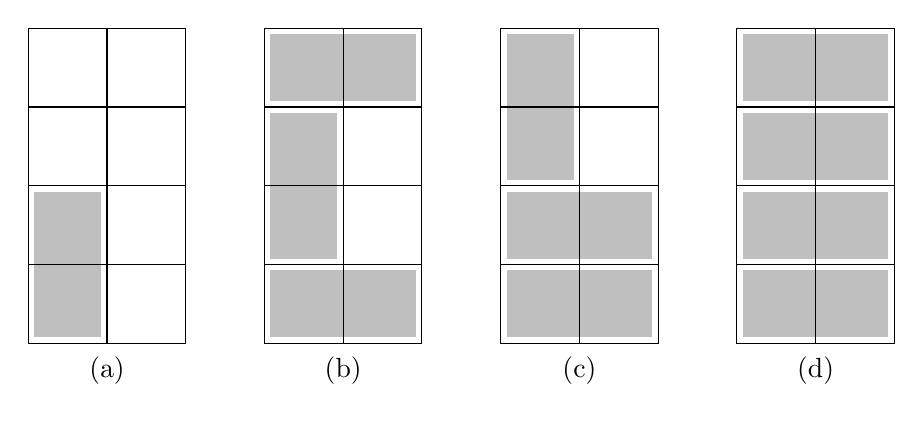
\begin{tikzpicture}
	[
		tile/.style = {shape=rectangle, fill=black!25, anchor=center},
		htile/.style = {tile, minimum width=1.85cm, minimum height=0.85cm},
		vtile/.style = {tile, minimum height=1.85cm, minimum width=0.85cm}	
	]
	
	\def\x{0}
	\def\y{0}
	
	\node [vtile] at ({\x + 0.5}, {\y + 1}) {};
	
	\draw (\x,\y) rectangle ({\x + 2}, {\y + 4});
	\draw ({\x + 1}, \y) -- ({\x + 1}, {\y + 4});
	\draw (\x, {\y + 1}) -- ({\x + 2}, {\y + 1});
	\draw (\x, {\y + 2}) -- ({\x + 2}, {\y + 2});
	\draw (\x, {\y + 3}) -- ({\x + 2}, {\y + 3});
	
	\node [yshift=-1em] at ({\x + 1}, \y) {(a)};
	
	\def\x{3}
	
	\node [htile] at ({\x + 1}, {\y + 0.5}) {};
	\node [vtile] at ({\x + 0.5}, {\y + 2}) {};
	\node [htile] at ({\x + 1}, {\y + 3.5}) {};
	
	\draw (\x,\y) rectangle ({\x + 2}, {\y + 4});
	\draw ({\x + 1}, \y) -- ({\x + 1}, {\y + 4});
	\draw (\x, {\y + 1}) -- ({\x + 2}, {\y + 1});
	\draw (\x, {\y + 2}) -- ({\x + 2}, {\y + 2});
	\draw (\x, {\y + 3}) -- ({\x + 2}, {\y + 3});
	
	\node [yshift=-1em] at ({\x + 1}, \y) {(b)};
	
	\def\x{6}
	
	\node [htile] at ({\x + 1}, {\y + 0.5}) {};
	\node [htile] at ({\x + 1}, {\y + 1.5}) {};
	\node [vtile] at ({\x + 0.5}, {\y + 3}) {};
	
	\draw (\x,\y) rectangle ({\x + 2}, {\y + 4});
	\draw ({\x + 1}, \y) -- ({\x + 1}, {\y + 4});
	\draw (\x, {\y + 1}) -- ({\x + 2}, {\y + 1});
	\draw (\x, {\y + 2}) -- ({\x + 2}, {\y + 2});
	\draw (\x, {\y + 3}) -- ({\x + 2}, {\y + 3});
	
	\node [yshift=-1em] at ({\x + 1}, \y) {(c)};
	
	\def\x{9}
	
	\node [htile] at ({\x + 1}, {\y + 0.5}) {};
	\node [htile] at ({\x + 1}, {\y + 1.5}) {};
	\node [htile] at ({\x + 1}, {\y + 2.5}) {};
	\node [htile] at ({\x + 1}, {\y + 3.5}) {};
	
	\draw (\x,\y) rectangle ({\x + 2}, {\y + 4});
	\draw ({\x + 1}, \y) -- ({\x + 1}, {\y + 4});
	\draw (\x, {\y + 1}) -- ({\x + 2}, {\y + 1});
	\draw (\x, {\y + 2}) -- ({\x + 2}, {\y + 2});
	\draw (\x, {\y + 3}) -- ({\x + 2}, {\y + 3});
	
	\node [yshift=-1em] at ({\x + 1}, \y) {(d)};
	
	
\end{tikzpicture}
			\caption{Four possible beginnings for a tiling of a $4\times(n+2)$ hallway.}
		\end{figure}
		The number of tilings with each beginning in Figure 3 are
		\begin{enumerate}
			\item $y(n+2)$
			\item $z(n+1)$
			\item $y(n+1)$
			\item $x(n)$
		\end{enumerate}
		It follows that $x(n+2) = x(n) + y(n+2) + y(n+1) + z(n+1)$.
		
		Now consider a $y$-hallway of length $n+1$. There are two possibilities for the leftmost two columns, shown in Figure 4. There are $x(n)$ tilings for the first possibility, and, by symmetry, $y(n)$ tilings for the second possibility. Thus, $y(n+1) = x(n) + y(n)$.
		\begin{figure}[H]
			\begin{center}
				
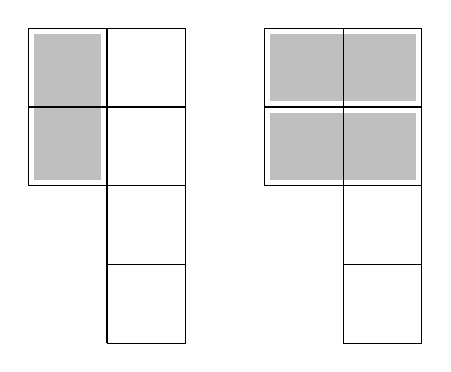
\begin{tikzpicture}
	[
		tile/.style = {shape=rectangle, fill=black!25, anchor=center},
		htile/.style = {tile, minimum width=1.85cm, minimum height=0.85cm},
		vtile/.style = {tile, minimum height=1.85cm, minimum width=0.85cm}	
	]
	
	\def\x{0}
	\def\y{0}
	
	\node [vtile] at ({\x + 0.5, \y + 3}) {};
	
	\draw ({\x + 1}, \y) -- ({\x + 2}, \y);
	\draw ({\x + 1}, {\y + 1}) -- ({\x + 2}, {\y + 1});
	\draw (\x, {\y + 2}) -- ({\x + 2}, {\y + 2});
	\draw (\x, {\y + 3}) -- ({\x + 2}, {\y + 3});
	\draw (\x, {\y + 4}) -- ({\x + 2}, {\y + 4});
	
	\draw (\x, {\y + 2}) -- (\x, {\y + 4});
	\draw ({\x + 1}, \y) -- ({\x + 1}, {\y + 4});
	\draw ({\x + 2}, \y) -- ({\x + 2}, {\y + 4});
	
	\def\x{3}
	
	\node [htile] at ({\x + 1}, {\y + 3.5}) {};
	\node [htile] at ({\x + 1}, {\y + 2.5}) {};
	
	\draw ({\x + 1}, \y) -- ({\x + 2}, \y);
	\draw ({\x + 1}, {\y + 1}) -- ({\x + 2}, {\y + 1});
	\draw (\x, {\y + 2}) -- ({\x + 2}, {\y + 2});
	\draw (\x, {\y + 3}) -- ({\x + 2}, {\y + 3});
	\draw (\x, {\y + 4}) -- ({\x + 2}, {\y + 4});
	
	\draw (\x, {\y + 2}) -- (\x, {\y + 4});
	\draw ({\x + 1}, \y) -- ({\x + 1}, {\y + 4});
	\draw ({\x + 2}, \y) -- ({\x + 2}, {\y + 4});
	
	
\end{tikzpicture}
			\end{center}
			\caption{Two possible beginnings for a tiling of a $y$-hallway of length $n+1$.}
		\end{figure}
		Finally, consider a $z$-hallway of length $n+2$. There are two possibilities for the leftmost three columns, shown in Figure 5. There are $x(n+1)$ tilings for the first possibility and $z(n)$ tilings for the second, so $z(n+2) = x(n+1) + z(n)$.
		\begin{figure}[H]
			\centering
			
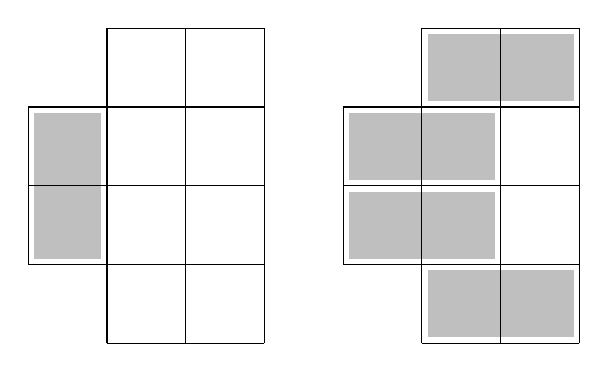
\begin{tikzpicture}
	[
		tile/.style = {shape=rectangle, fill=black!25, anchor=center},
		htile/.style = {tile, minimum width=1.85cm, minimum height=0.85cm},
		vtile/.style = {tile, minimum height=1.85cm, minimum width=0.85cm}	
	]
	
	\def\x{0}
	\def\y{0}
	
	\node [vtile] at ({\x + 0.5}, {\y + 2}) {};
	
	\draw ({\x + 1}, \y) -- ({\x + 3}, \y);
	\draw (\x, {\y + 1}) -- ({\x + 3}, {\y + 1});
	\draw (\x, {\y + 2}) -- ({\x + 3}, {\y + 2});
	\draw (\x, {\y + 3}) -- ({\x + 3}, {\y + 3});
	\draw ({\x + 1}, {\y + 4}) -- ({\x + 3}, {\y + 4});
	
	\draw (\x, {\y + 1}) -- (\x, {\y + 3});
	\draw ({\x + 1}, \y) -- ({\x + 1}, {\y + 4});
	\draw ({\x + 2}, \y) -- ({\x + 2}, {\y + 4});
	\draw ({\x + 3}, \y) -- ({\x + 3}, {\y + 4});
	
	\def\x{4}
	
	\node [htile] at ({\x + 1}, {\y + 1.5}) {};
	\node [htile] at ({\x + 1}, {\y + 2.5}) {};
	\node [htile] at ({\x + 2}, {\y + 0.5}) {};
	\node [htile] at ({\x + 2}, {\y + 3.5}) {};
	
	\draw ({\x + 1}, \y) -- ({\x + 3}, \y);
	\draw (\x, {\y + 1}) -- ({\x + 3}, {\y + 1});
	\draw (\x, {\y + 2}) -- ({\x + 3}, {\y + 2});
	\draw (\x, {\y + 3}) -- ({\x + 3}, {\y + 3});
	\draw ({\x + 1}, {\y + 4}) -- ({\x + 3}, {\y + 4});
	
	\draw (\x, {\y + 1}) -- (\x, {\y + 3});
	\draw ({\x + 1}, \y) -- ({\x + 1}, {\y + 4});
	\draw ({\x + 2}, \y) -- ({\x + 2}, {\y + 4});
	\draw ({\x + 3}, \y) -- ({\x + 3}, {\y + 4});
	
	
\end{tikzpicture}
			\caption{Two possible beginnings for a tiling of a $z$-hallway of length $n+2$.}
		\end{figure}
	
		This gives the system of three equations
		\begin{equation*}
			\begin{aligned}
				x(n+2) &= x(n) + y(n+2) + y(n+1) + z(n+1) \\
				y(n+1) &= x(n) + y(n) \\
				z(n+2) &= x(n+1) + z(n)
			\end{aligned}
		\end{equation*}
	
		\questionpart It is obvious that $x(1) = 1$, $y(1) = 1$, and $z(1) = 1$. Figure 6 shows the possible tilings of a $4\times 2$ hallway, a $y$-hallway of length 2, and a $z$-hallway of length 2.
		\begin{figure}[H]
			\centering
			
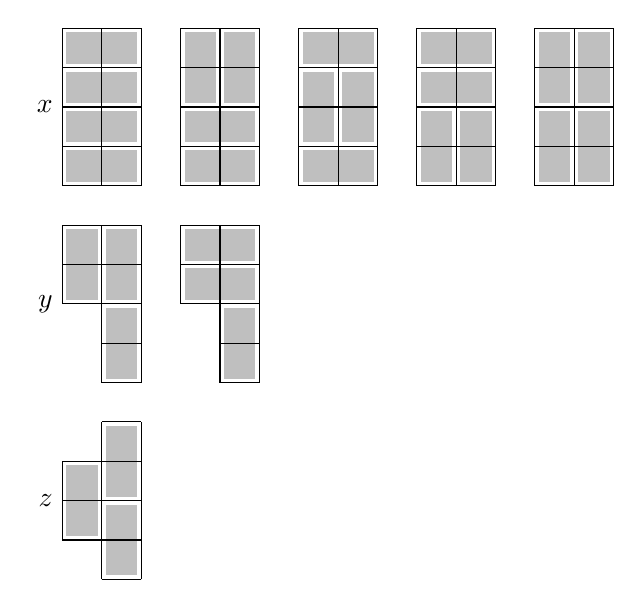
\begin{tikzpicture}
	[
		scale = .5, thin,
		tile/.style = {shape=rectangle, fill=black!25, anchor=center},
		htile/.style = {tile, minimum width=0.9cm, minimum height=0.4cm},
		vtile/.style = {tile, minimum height=0.9cm, minimum width=0.4cm}	
	]
	
	\def\x{0}
	\def\y{0}
	
	\node [anchor=east] at (\x, {\y + 2}) {$x$};
	
	\newcommand{\htile}[2]{\node [htile] at ({\x + #1}, {\y + #2 + .5}) {}; }
	\newcommand{\vtile}[2]{\node [vtile] at ({\x + #1 + .5}, {\y + #2}) {}; }
	
	\foreach \h in {0, 1, 2, 3} {\htile{1}{\h}}
	
	\foreach \h in {0, 1, 2, 3, 4} { \draw (\x, {\y + \h}) -- ({\x + 2}, {\y + \h}); }
	\draw (\x, \y) -- (\x, {\y + 4});
	\draw ({\x + 1}, \y) -- ({\x + 1}, {\y + 4});
	\draw ({\x + 2}, \y) -- ({\x + 2}, {\y + 4});
	
	\def\x{3}
	
	\htile{1}{0}
	\htile{1}{1}
	\vtile{0}{3}
	\vtile{1}{3}
	
	\foreach \h in {0, 1, 2, 3, 4} { \draw (\x, {\y + \h}) -- ({\x + 2}, {\y + \h}); }
	\draw (\x, \y) -- (\x, {\y + 4});
	\draw ({\x + 1}, \y) -- ({\x + 1}, {\y + 4});
	\draw ({\x + 2}, \y) -- ({\x + 2}, {\y + 4});
	
	\def\x{6}
	
	\htile{1}{0}
	\vtile{0}{2}
	\vtile{1}{2}
	\htile{1}{3}
	
	\foreach \h in {0, 1, 2, 3, 4} { \draw (\x, {\y + \h}) -- ({\x + 2}, {\y + \h}); }
	\draw (\x, \y) -- (\x, {\y + 4});
	\draw ({\x + 1}, \y) -- ({\x + 1}, {\y + 4});
	\draw ({\x + 2}, \y) -- ({\x + 2}, {\y + 4});
	
	\def\x{9}
	
	\vtile{0}{1}
	\vtile{1}{1}
	\htile{1}{2}
	\htile{1}{3}
	
	\foreach \h in {0, 1, 2, 3, 4} { \draw (\x, {\y + \h}) -- ({\x + 2}, {\y + \h}); }
	\draw (\x, \y) -- (\x, {\y + 4});
	\draw ({\x + 1}, \y) -- ({\x + 1}, {\y + 4});
	\draw ({\x + 2}, \y) -- ({\x + 2}, {\y + 4});
	
	\def\x{12}
	
	\vtile{0}{1}
	\vtile{1}{1}
	\vtile{0}{3}
	\vtile{1}{3}
	
	\foreach \h in {0, 1, 2, 3, 4} { \draw (\x, {\y + \h}) -- ({\x + 2}, {\y + \h}); }
	\draw (\x, \y) -- (\x, {\y + 4});
	\draw ({\x + 1}, \y) -- ({\x + 1}, {\y + 4});
	\draw ({\x + 2}, \y) -- ({\x + 2}, {\y + 4});
	
	\def\y{-5}
	\def\x{0}
	\node [anchor=east] at (\x, {\y + 2}) {$y$};
	
	\vtile{0}{3}
	\vtile{1}{3}
	\vtile{1}{1}
	
	\foreach \h in {0, 1} { \draw  ({\x + 1}, {\y + \h}) -- ({\x + 2}, {\y + \h}); }
	\foreach \h in {2, 3, 4} { \draw (\x, {\y + \h}) -- ({\x + 2}, {\y + \h}); }
	
	\draw (\x, {\y + 2}) -- (\x, {\y + 4});
	\draw ({\x + 1}, \y) -- ({\x + 1}, {\y + 4});
	\draw ({\x + 2}, \y) -- ({\x + 2}, {\y + 4});
	
	\def\x{3}
	
	\htile{1}{3}
	\htile{1}{2}
	\vtile{1}{1}
	
	\foreach \h in {0, 1} { \draw  ({\x + 1}, {\y + \h}) -- ({\x + 2}, {\y + \h}); }
	\foreach \h in {2, 3, 4} { \draw (\x, {\y + \h}) -- ({\x + 2}, {\y + \h}); }
	
	\draw (\x, {\y + 2}) -- (\x, {\y + 4});
	\draw ({\x + 1}, \y) -- ({\x + 1}, {\y + 4});
	\draw ({\x + 2}, \y) -- ({\x + 2}, {\y + 4});
	
	\def\y{-10}
	\def\x{0}
	\node [anchor=east] at (\x, {\y + 2}) {$z$};
	
	\vtile{0}{2}
	\vtile{1}{3}
	\vtile{1}{1}
	
	\foreach \h in {0, 4} { \draw  ({\x + 1}, {\y + \h}) -- ({\x + 2}, {\y + \h}); }
	\foreach \h in {1, 2, 3} { \draw (\x, {\y + \h}) -- ({\x + 2}, {\y + \h}); }
	
	\draw (\x, {\y + 1}) -- (\x, {\y + 3});
	\draw ({\x + 1}, \y) -- ({\x + 1}, {\y + 4});
	\draw ({\x + 2}, \y) -- ({\x + 2}, {\y + 4});
\end{tikzpicture}

			\caption{The possible tilings of a hallway, $y$-hallway, and $z$-hallway of length 2.}
		\end{figure}
		It is easy to see from this that $x(2) = 5$, $y(2) =2$, and $z(2) =1$. We can use the system from (a) and these initial conditions to compute $x(10)=18061$; see the table of values obtained by iteratively applying the system in Table 1.
		
		\begin{table}[H]
			\centering
			\begin{tabular}{@{}l|llllllllll@{}}
				$n$ & 1 & 2 & 3 & 4 & 5 & 6 & 7 & 8 & 9 & 10 \\
				\midrule
				$x(n)$ & 1 & 5 & 11 & 36 & 95 & 281 & 781 & 2245 & 6336 & 18061  \\
				$y(n)$ & 1 & 2 & 7 & 18 & 54 & 149 & 430 & 1211 & 3456 & 9792  \\
				$z(n)$ & 1 & 1 & 6 & 12 & 42 & 107 & 323 & 888 & 2568 & 7224  \\
			\end{tabular}
			\caption{Computed values of $x(n)$, $y(n)$, and $z(n)$ for $n = 1,2,\dots,10$.}
		\end{table}
		
	\end{alphaparts}
	
	\question*{3.75} Summing the three equations gives
	\begin{equation*}
		\Delta x(t) + \Delta y(t) + \Delta z(t) = -x(t) + \frac{1}{3}y(t) + \frac{2}{3}z(t) + \frac{1}{3}x(t) - \frac{1}{3}y(t) + \frac{1}{3}z(t) + \frac{2}{3}x(t) -z(t) = 0
	\end{equation*}
	so $x(t) + y(t) + z(t) = \text{constant}$ because we are working over $t=0,1,2,\dots$ Since, initially, $x(0) = .5$, $y(0) = .3$, and $z(0) = .2$, we must have $x(t) + y(t) +z(t) = 1$ for all $t$. Substituting $z(t) = 1 - x(t) - y(t)$ into the original equations gives
	\begin{equation*}
		\begin{aligned}
			\Delta x(t) &= -x(t) + \frac{1}{3}y(t) + \frac{2}{3}(1-x(t) - y(t)) = -\frac{5}{3}x(t)-\frac{1}{3}y(t) + \frac{2}{3} \\
			\Delta y(t) &= \frac{1}{3}x(t) -\frac{1}{3}y(t) +\frac{1}{3}(1-x(t)-y(t)) = -\frac{2}{3}y(t) + \frac{1}{3}
		\end{aligned}
	\end{equation*}
	The second equation is the same as $y(t+1) - \frac{1}{3}y(t) = \frac{1}{3}$. Since $u(t) = \left(\frac{1}{3}\right)^t$ is a solution of the homogeneous equation $u(t+1) - \frac{1}{3}u(t) = 0$, and $y_p(t) = \frac{1}{2}$ is a solution of the equation for $y$, a general solution for $y(t)$ is $y(t) = \frac{1}{2} + c\left(\frac{1}{3}\right)^t$, for some constant $c$.
	
	Plugging in to the $x(t)$ equation above gives
	\begin{equation*}
		x(t+1) + \frac{2}{3}x(t) = -\frac{1}{3}\left(\frac{1}{2} + c\left(\frac{1}{3}\right)^t\right) + \frac{2}{3} = \frac{1}{2} - c\left(\frac{1}{3}\right)^{t+1}
	\end{equation*}
	Then $u(t) = \left(-\frac{2}{3}\right)^t$ is a solution of the homogeneous equation $u(t+1) + \frac{2}{3}u(t) = 0$, and
	\begin{equation*}
		\begin{aligned}
			x(t) &= u(t) \sum \frac{\frac{1}{2} - c\left(\frac{1}{3}\right)^{t+1}}{u(t+1)} = \left(-\frac{2}{3}\right)^t\sum\frac{\frac{1}{2} - c\left(\frac{1}{3}\right)^{t+1}}{\left(-\frac{2}{3}\right)^{t+1}}\\
			&= -\frac{3}{2}\cdot\left(-\frac{2}{3}\right)^t\sum \left[\frac{1}{2}\cdot\left(-\frac{3}{2}\right)^t - \frac{c}{3}\cdot\left(-\frac{1}{2}\right)^t\right] \\
			&= -\frac{3}{2}\cdot\left(-\frac{2}{3}\right)^t\left[\frac{1}{2}\cdot\frac{1}{-\frac{3}{2} - 1}\cdot\left(-\frac{3}{2}\right)^t - \frac{c}{3}\cdot\frac{1}{-\frac{1}{2} - 1}\cdot\left(-\frac{1}{2}\right)^t + d'\right] \\
			&= \frac{3}{10} - \frac{c}{3}\cdot\left(\frac{1}{3}\right)^t + d\left(-\frac{2}{3}\right)^t
		\end{aligned}
	\end{equation*}
	for some constants $d,d'$. Applying the initial conditions $x(0) = .5$ and $y(0) = .3$, we get $c = -\frac{1}{5}$ and $d=\frac{2}{15}$.
	
	
	Therefore, the solution of the original equations is
	\begin{equation*}
		\begin{aligned}
			x(t) &= \frac{3}{10} + \frac{1}{15}\left(\frac{1}{3}\right)^t + \frac{2}{15}\left(-\frac{2}{3}\right)^t\\
			y(t) &= \frac{1}{2} - \frac{1}{5}\left(\frac{1}{3}\right)^t \\
			z(t) &= \frac{1}{5} + \frac{2}{15}\left(\frac{1}{3}\right)^t - \frac{2}{15}\left(-\frac{2}{3}\right)^t
		\end{aligned}
	\end{equation*}

	\newcommand{\awin}{\mathcal{A}}
	\newcommand{\bwin}{\mathcal{B}}
	\newcommand{\nowin}{\mathcal{N}}
	\newcommand{\chips}[2]{[#1,#2]}
	\question*{3.76} 
	\begin{alphaparts}
		\questionpart Let $\mathcal{A}$ be the event that $A$ wins, let $\mathcal{B}$ be the event that $B$ wins, and let $\mathcal{N}$ be the event that neither wins (the game goes on forever). Let $\chips{n}{t}$ be the event that player $A$ has $t$ chips on turn $n$.
		
		All probabilities conditioned on the state of the game at turn $n$ depend only on how many chips each player has at turn $n$, rather than the exact history of the game. Assuming a fixed total number of chips, any probability conditioned on the state of the game at turn $n$ actually depends only on the number of chips $t$ that player $A$ has on turn $n$ (since $B$ must have the total minus $t$ chips). Hence, the function $u(t) = P(\awin \mid \chips{n}{t}, \chips{n_1}{t_1}, \dots, \chips{t_k}{n_k})$ for any $n > n_1 > \cdots > n_k$ is well-defined.
		
		As long as $t$ is not 0 or the total number of chips, then conditioning on the complementary events $\chips{n+1}{t-1} \mid \chips{n}{t}$ and $\chips{n+1}{t+1} \mid \chips{n}{t}$ allows us to write
		\begin{equation*}
			\begin{aligned}
				P(\mathcal{A} \mid \chips{n}{t}) &= P(\mathcal{A} \mid \chips{n+1}{t-1}, \chips{n}{t})P(\chips{n+1}{t-1} \mid \chips{n}{t}) \\
				&+ P(\mathcal{A} \mid \chips{n+1}{t+1}, \chips{n}{t}) P(\chips{n+1}{t+1} \mid \chips{n}{t})
			\end{aligned}
		\end{equation*}
		which implies that
		\begin{equation*}
			\begin{aligned}
				u(t) &= u(t-1)P(\chips{n+1}{t-1} \mid \chips{n}{t}) + u(t+1)P(\chips{n+1}{t+1}\mid \chips{n}{t}) \\
				&= (1-p)u(t-1) + pu(t+1)
			\end{aligned}
		\end{equation*}
		because by assumption $P(\chips{n+1}{t-1}\mid\chips{n}{t}) = 1-p$, and $P(\chips{n+1}{t+1}\mid\chips{n}{t}) = p$.
		
		\questionpart Suppose that at the beginning of the game $A$ has $a$ chips and $B$ has $b$ chips. Suppose that $A$ wins on turn $n$; then we have
		\begin{equation*}
			u(a + b) = P(\awin \mid \chips{n}{a+b}) = 1
		\end{equation*}
		Now suppose that $A$ loses on turn $n$; then we have
		\begin{equation*}
			u(0) = P(\awin \mid \chips{n}{0}) = 0
		\end{equation*}
		Assume that $p\ne 0$. Rewriting the difference equation from above gives
		\begin{equation*}
			u(t+2) - \frac{1}{p}u(t+1) + \frac{1-p}{p}u(t) = 0
		\end{equation*}
		which has characteristic equation $\lambda^2 - \frac{1}{p}\lambda + \frac{1-p}{p}= 0$. This equation has roots
		$\lambda = 1, \frac{1}{p} -1$, so a general solution of the difference equation is
		\begin{equation*}
			u(t) = c_1 + c_2\left(\frac{1}{p} - 1\right)^t
		\end{equation*}
		for constants $c_1$ and $c_2$. Using the condition $u(0) = 0$ gives $c_1  = -c_2$, and $u(t) = c_1\left[1-\left(\frac{1}{p}-1\right)^t\right]$. Applying the condition $u(a+b) = 1$ gives $c_1 = \frac{1}{1-\left(\frac{1}{p}-1\right)^{a+b}}$, so
		\begin{equation*}
			u(t) = \frac{1-\left(\frac{1}{p}-1\right)^t}{1-\left(\frac{1}{p} - 1\right)^{a+b}}
		\end{equation*}
		Finally, the probability that $A$ wins is just
		\begin{equation*}
			P(\awin) = P(\awin \mid [1, a]) = u(a) = \frac{1-\left(\frac{1}{p} - 1\right)^a}{1-\left(\frac{1}{p} - 1\right)^{a+b}}
		\end{equation*}
		Note: using symmetry to obtain $P(\bwin)$ shows that $P(\bwin) = 1 - P(\awin)$, which implies that $P(\nowin) = 0$, that is, the game must eventually end after finitely many turns.
	
	\end{alphaparts}
	
\end{document}